\chapter{\xlabel{pol2_image}POL-2 Image Display}
\label{sec:display}

\section{\xlabel{gaia}GAIA}

The \starlink\ package \gaia\ can be used to inspect the results of
the data reduction.  To plot the output vector catalogue onto the
final total intensity map first open up the I map in \GAIA.

\begin{terminalv}
% gaia iext.sdf
\end{terminalv}


In the main \GAIA\ window, select the drop-down menu option
\texttt{Image Analysis / Polarimetry toolbox…}. This should launch a
new toolbox window entitled GAIA: Polarimetry. From this window, use
the drop-down menu option \texttt{File / Open} to load the file
\file{mycat.FIT}. This should then populate the lower part of the window
with the contents of this polarimetry catalogue file.  Each of the vectors
in this file will be automatically overlaid on the main image window
(see Figure \ref{fig:gaiavectorsopen}).

\begin{figure}[t!]
\begin{center}
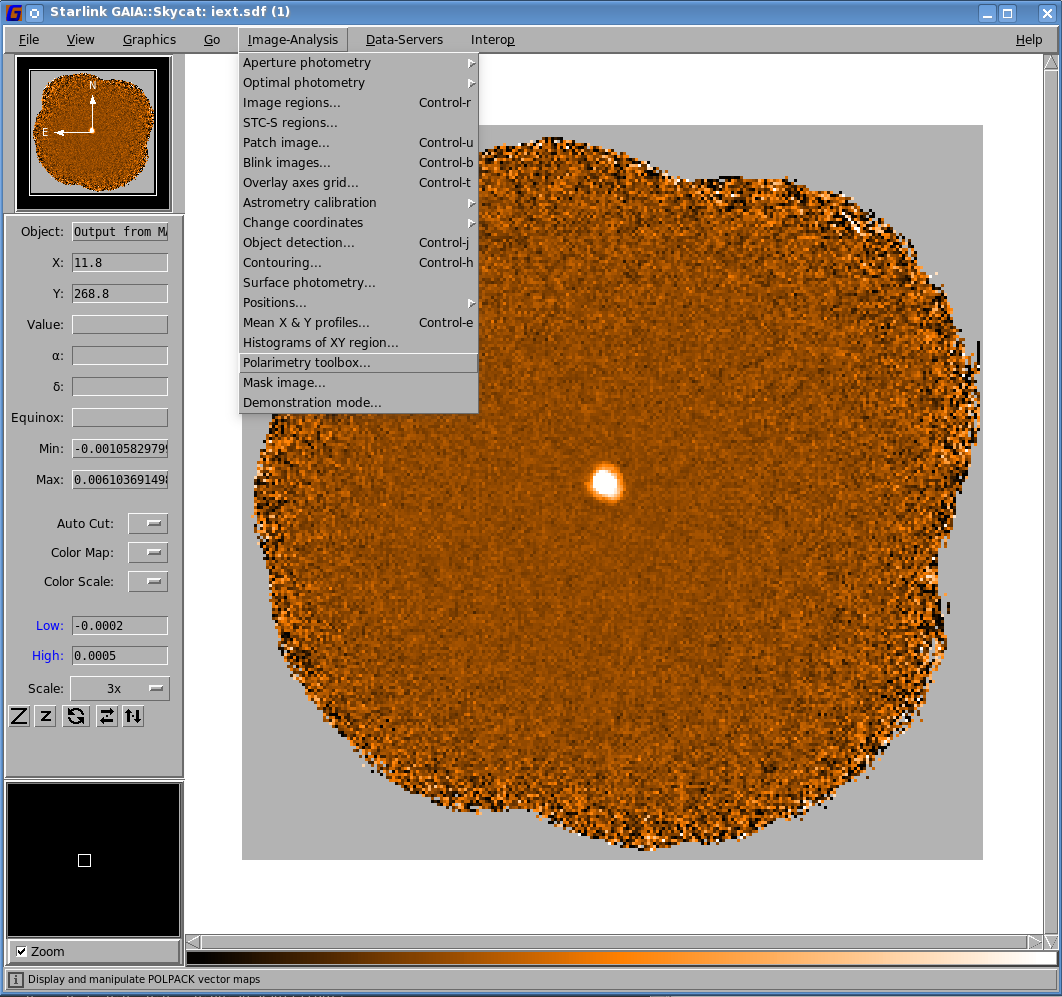
\includegraphics[width=0.46\linewidth]{sc22-gaia-plot-vectors-1.png}
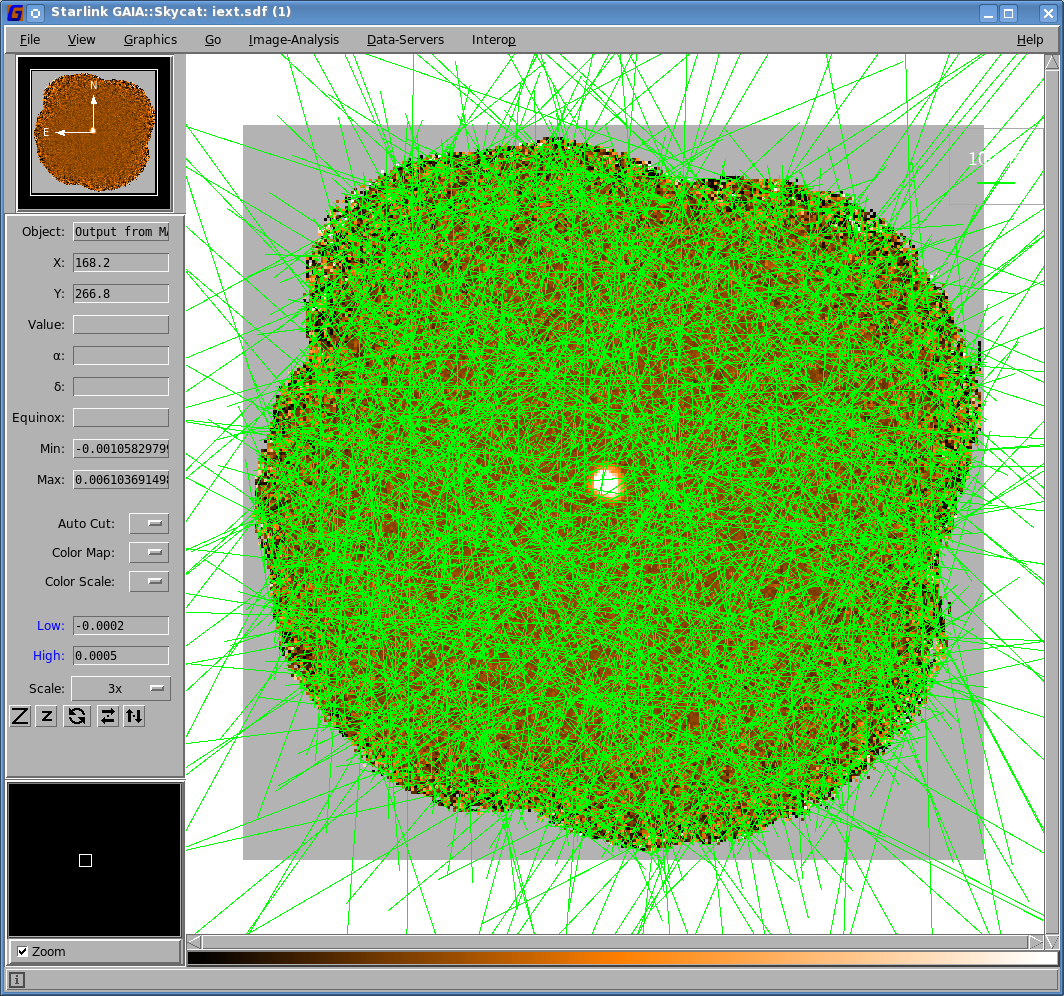
\includegraphics[width=0.46\linewidth]{sc22-gaia-plot-vectors-3.png}
\caption [Over Plotting Vectors in GAIA]{
  Left: Opening up the polarimetry toolbox in \GAIA. Right: The initial POL-2
  vectors overplotted in \GAIA.
\label{fig:gaiavectorsopen}
}
\end{center}
\end{figure}

In order to filter the number of overlaid vectors down to a more
useful number and size, you can use various options in the
\texttt{GAIA: Polarimetry} toolbox can be used. First, select the
\texttt{Rendering} tab on the
left hand side. This will reveal a panel that will indicate which
quantities are currently being used for the vector overlays. In this
case, the Vector length is taken from the P column of the table, and
the Vector angles are taken from the ANG column.

Currently the figure has too many vectors to be scientifically
meaningful. To filter out most of the extraneous vectors, click on the
Selecting tab, and set the Expression field to be the following:

\begin{terminalv}
$I/$DI<10
\end{terminalv}

\emph{Ensure you press return after entering in the above expression}.

The above expression selects the data points in the polarimetry table
which have an associated total intensity (column I) less than 10 times
the associated error value for that intensity (column DI). To remove
all of these extraneous vectors, either press control-X or use the
drop-down menu option \texttt{Edit / Cut}.  This should leave just a
small number of vectors clustering around the target object (see
Figure \ref{fig:gaiavectorssecond}).

\begin{figure}[t!]
\begin{center}
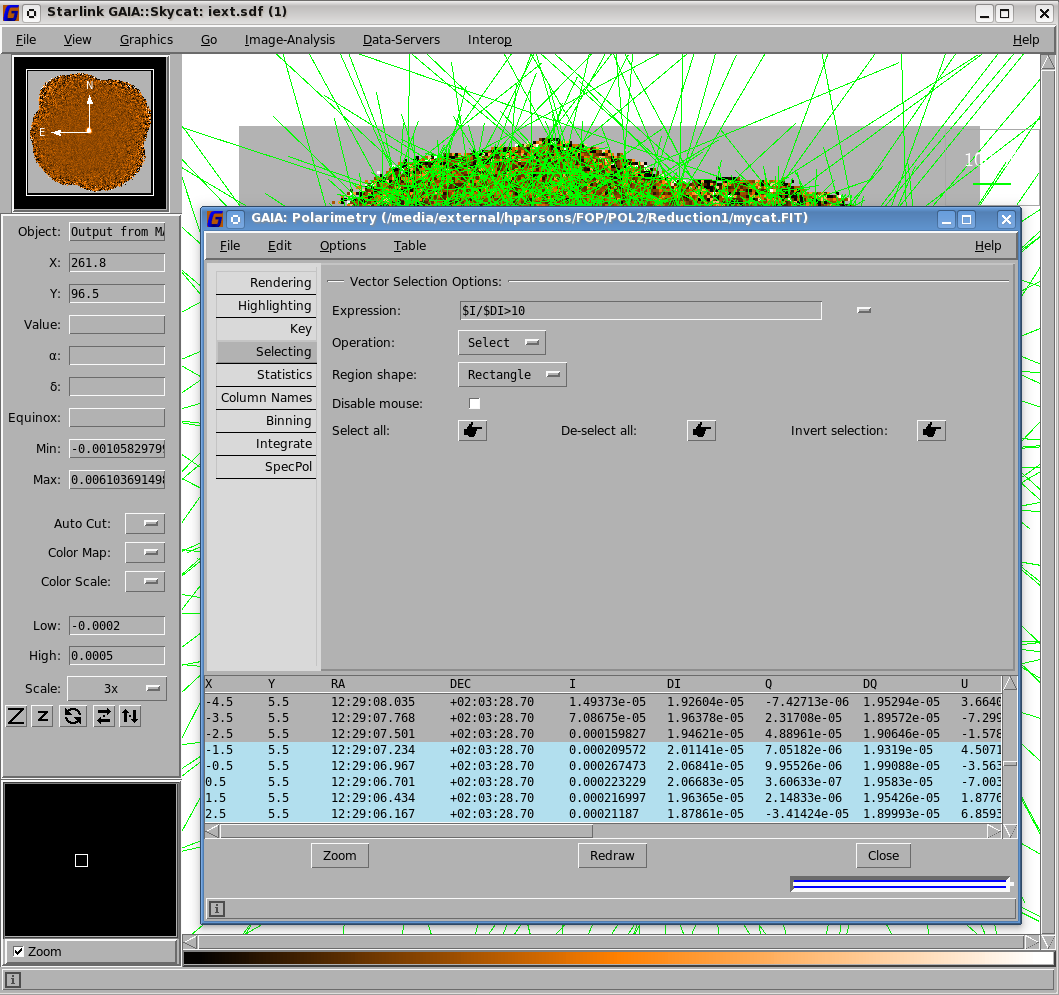
\includegraphics[width=0.46\linewidth]{sc22-gaia-plot-vectors-4.png}
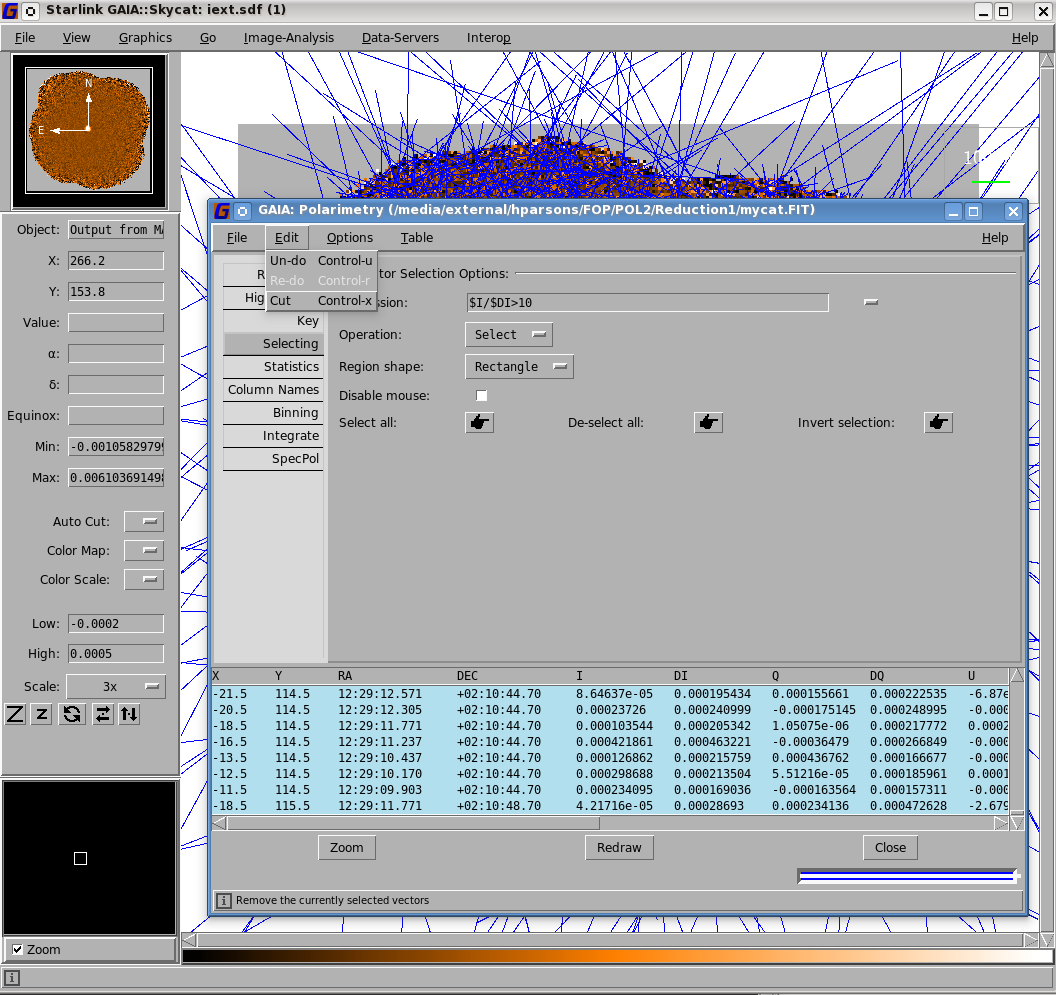
\includegraphics[width=0.46\linewidth]{sc22-gaia-plot-vectors-6.png}
\caption [Selecting Vectors in GAIA]{Left: specifying vectors
  to display via the expression \$I/\$DI$>$10. This will only plot
  vectors with an \SI{850}{\micro\metre} intensity signal-to-noise
  ratio greater than 10 in \GAIA. To ensure that this is specified,
  ensure you press the carriage return after entering the expression.
}
\label{fig:gaiavectorssecond}
\end{center}
\end{figure}

Zooming in on the central region of the map, it can already be seen
that the level of vector ordering (and hence polarisation) is quite
low (see Figure \ref{fig:gaiavectorsfinal}). If needed it is
possible to change the scaling by selecting the Rendering tab in the
GAIA: Polarimetry window, and increasing the vector scale.


\begin{figure}[t!]
\begin{center}
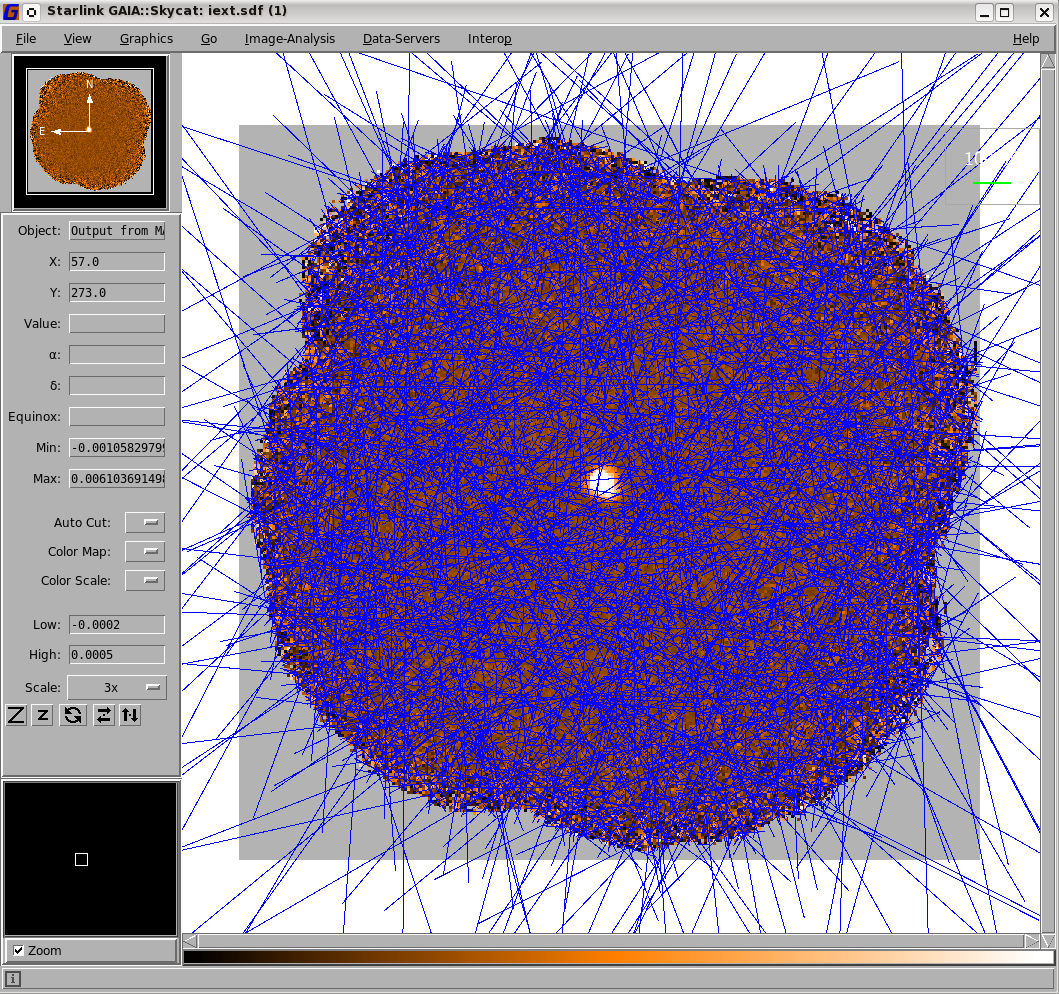
\includegraphics[width=0.44\linewidth]{sc22-gaia-plot-vectors-5.png}
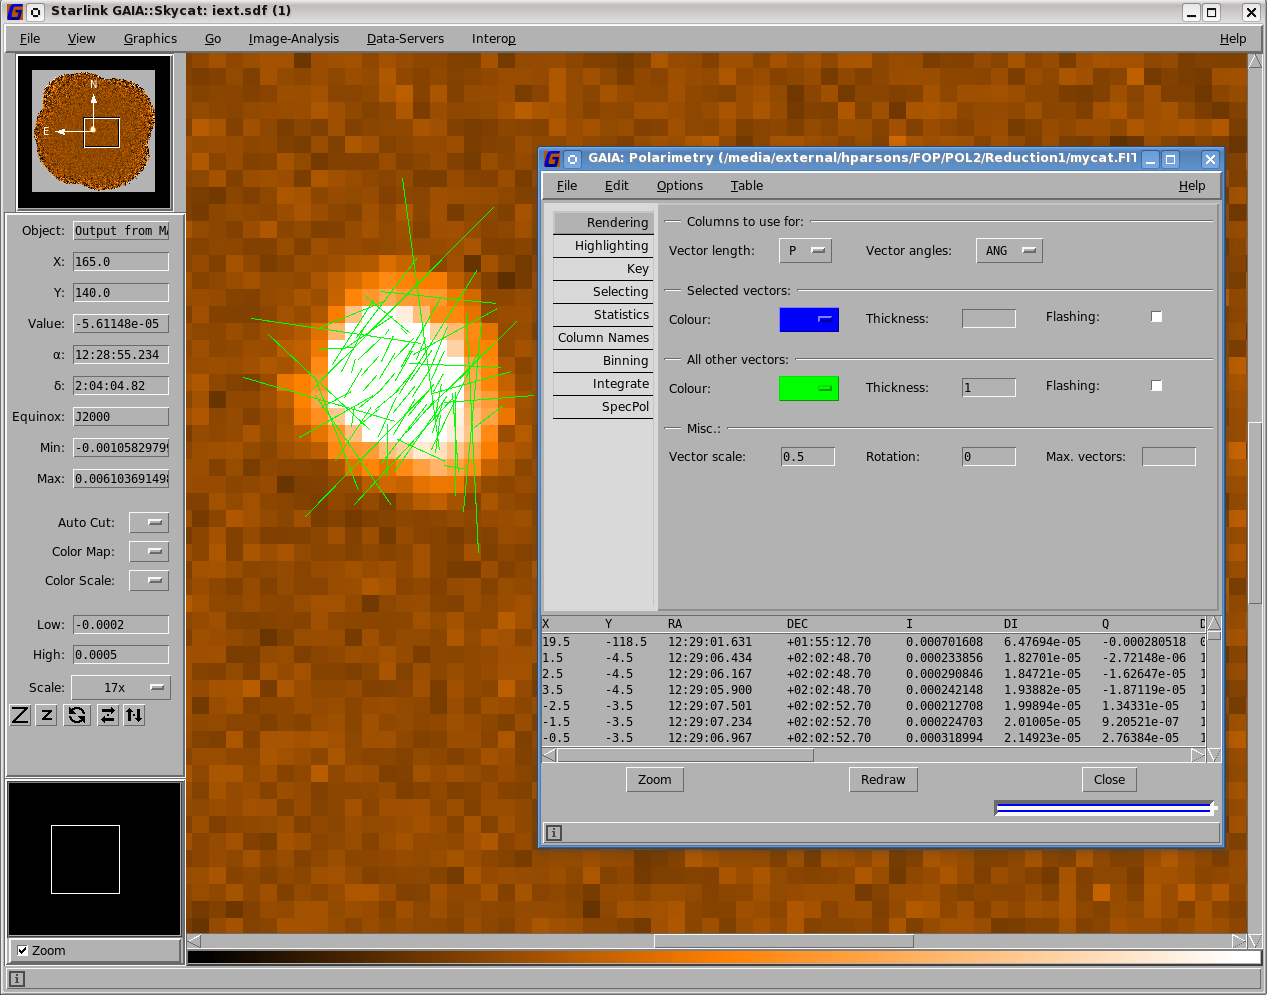
\includegraphics[width=0.52\linewidth]{sc22-gaia-plot-vectors-7.png}
\caption [Over Plotting Vectors in GAIA]{ Left: Selected vectors are
  marked in blue in this example, Right: after removal of selected
  vectors all that remains are the vectors on the (zoomed) regions
  where \$I/\$DI $>$ 10.}
\label{fig:gaiavectorsfinal}
\end{center}
\end{figure}


Finally it is useful for future use (as in the examples in the
following sections) to save the final selection of vectors. To save the
displayed vectors to a new catalogue, use the drop-down menu
\texttt{File / Save} in the polarimetry toolbox.

\section{\xlabel{kappa}KAPPA and polpack}

It is possible to use \Kappa\ and \polpack\ to create POL-2 plots.

\begin{terminalv}
% kappa
% polpack
\end{terminalv}

Note that in the following examples, it will be necessary to ensure
that only the vectors to be plotted are included in the file
\file{mycat.FIT}.

There are two main ways to do this - either by saving the output
catalogue from \GAIA\ or using the Starlink package
\xref{\textsc{CURSA}}{sun190}{} to manipulate
the catalogue you produced.  To use \textsc{CURSA} simply run:

\begin{terminalv}
% cursa
\end{terminalv}

then to select the vectors of interest:

\begin{terminalv}
% catselect catin=mycat.FIT catout=selcat.FIT norejcat seltyp=e "expr='i>10*di'"
\end{terminalv}

it is also possible to crop images using catselect, by using the
expression command.  In this example we use only pixels above -10 on
the y axis.

\begin{terminalv}
% catselect catin=mycat.FIT catout=selcat.FIT norejcat seltyp=e "expr='i>10*di and y>-10'"
\end{terminalv}




\begin{tip}
  For a better font on pgplot postscript devices, set the following
  environment variable.

\begin{terminalv}
setenv PGPLOT_PS_FONT Times
\end{terminalv}

For more info, see
\url{http://pipelinesandarchives.blogspot.com/2015/02/better-fonts-in-postscript-output-from.html}

Graphics-related attributes that can be set are described in
\xref{SUN95: Descriptions of Plotting
  Attributes}{sun95}{ap_plotting_attr}, and the coordinate system attributes that can be set are
described in \xref{SUN/95: Descriptions of Frame Attributes}{sun95}{ap_frmatt}.
\end{tip}





\subsection{\xlabel{kappa-example1} Example 1 -- a vector map with no background}
\label{section:kappa-example1}

In this section an output file: \file{plot1.pdf} is created from the input
catalogue \file{mycat.FIT}

Select the PostScript graphics device, writing to file \file{plot1.ps}.

\begin{terminalv}
gdset plot1.ps/acps
\end{terminalv}

For convenience, create a text file holding the main plotting style for
\task{polplot}.

\begin{terminalv}
% cat sty
colour = black
drawtitle=0
format(1)=hms
format(2)=dms
\end{terminalv}

Likewise, create a text file holding the style for the vector length key:

\begin{terminalv}
% cat ksty
colour = black
drawtitle=0
\end{terminalv}


Plot the vector map (the \texttt{vscale} parameter controls the vector
scale, and the \texttt{keyvec} parameter controls the length of the
vector used as the key. There are many other parameters that can be
used to control the behaviour of \texttt{polplot} -- see the \polpack
manual (SUN/223).

\begin{terminalv}
% polplot selcat.FIT  style=^sty keystyle=^ksty vscale=20 keyvec=20
\end{terminalv}

Convert the map into PDF file and remove blank margins (if required):

\begin{terminalv}
% ps2pdf plot1.ps temp.pdf
% pdfcrop temp.pdf plot1.pdf
\end{terminalv}


\begin{figure}[t!]
\begin{center}
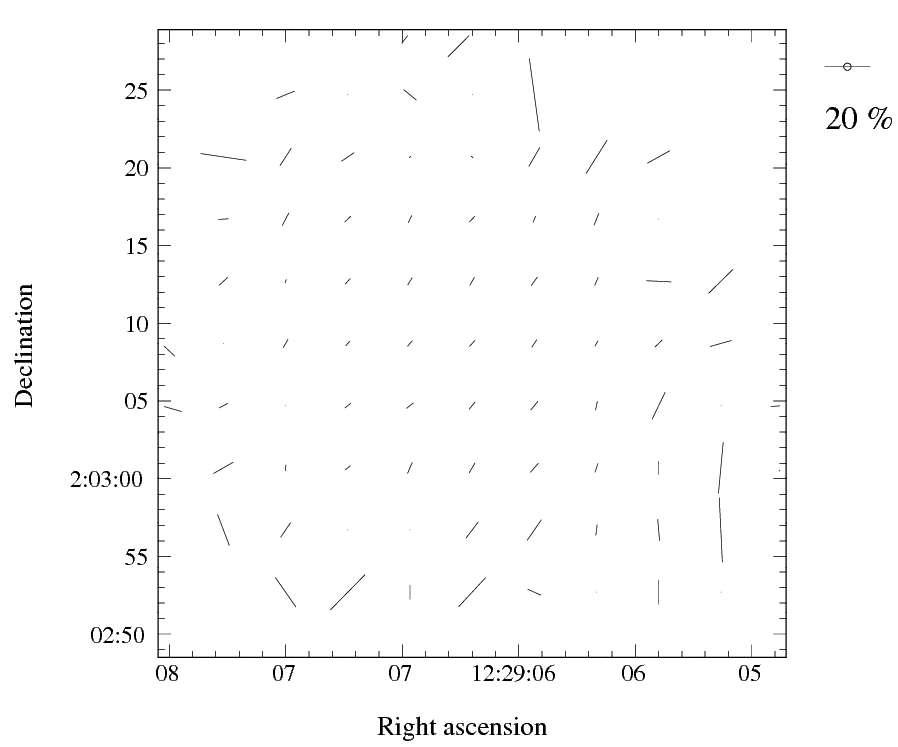
\includegraphics[width=0.75\linewidth]{sc22-kappa-plots-plot1.png}
\caption [Vector map with polplot]{ Result from Example 1: Producing a
  vector map with no background using \task{polplot}.}
\label{fig:kappa-plot1}
\end{center}
\end{figure}

\subsection{\xlabel{kappa-example2} Example 2 -- a vector map over a contour map}
\label{section:kappa-example2}


In this section we create an output file: \file{plot2.pdf} from the input
catalogue \file{mycat.FIT}.

\begin{terminalv}
% gdset plot2.ps/acps
\end{terminalv}

Setting up the main plotting style for \contour\ and \task{polplot}:

\begin{terminalv}
% cat sty
colour = black
colour(curves)=red
width(curves)=3
drawtitle=0
format(1)=hms
format(2)=dms
\end{terminalv}


Produce the contour map

\begin{terminalv}
% contour iext\(0~150,0~200\) mode=perc percentiles=\[88,90,92,94,96,98\] style=^sty key=no
\end{terminalv}


Modify the above style for the vector map to produce black vectors

\begin{terminalv}
% cat vsty
^sty
colour(curves)=black
\end{terminalv}


Set the style for the vector length key:


\begin{terminalv}
% cat ksty
colour=black
width=3
drawtitle=0
\end{terminalv}

Plot the vector map over the contour map. The vectors and contours are
aligned automatically in sky coordinates:


\begin{terminalv}
% polplot selcat.FIT axes=no clear=no style=^vsty keystyle=^ksty vscale=20 keyvec=20
\end{terminalv}

Convert into a PDF file and remove blank margins (if required):

\begin{terminalv}
% ps2pdf plot2.ps temp.pdf
% pdfcrop temp.pdf plot2.pdf
\end{terminalv}

\begin{figure}[t!]
\begin{center}
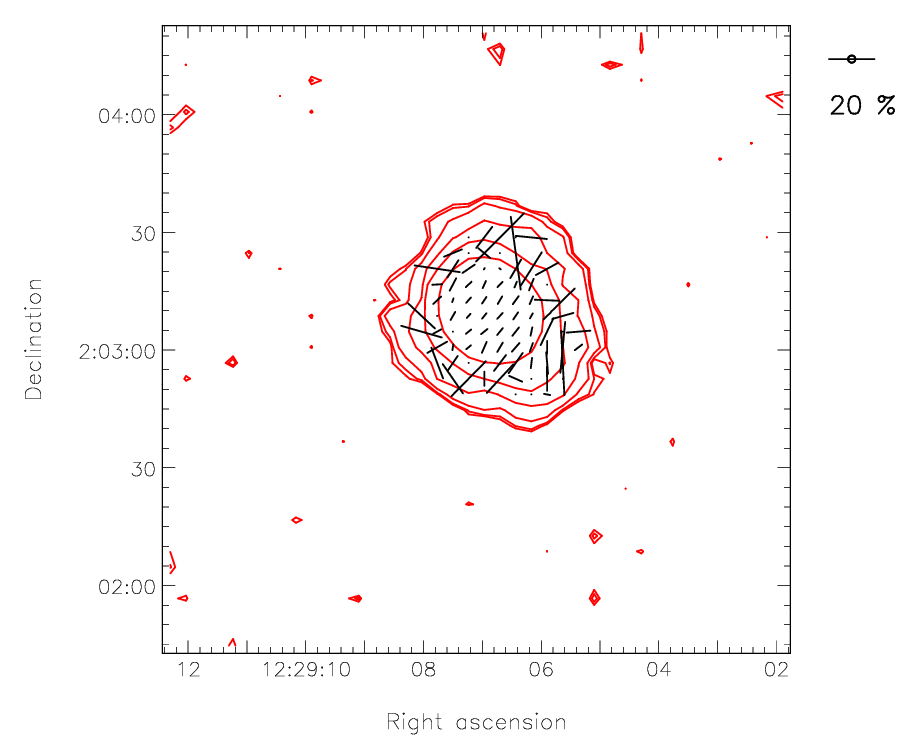
\includegraphics[width=0.75\linewidth]{sc22-kappa-plots-plot2.png}

\caption [Vector map with contour map in polplot]{Result from Example
  1: Producing a vector map over a contour map.\label{fig:kappa-plot2}}
\end{center}
\end{figure}

\subsection{\xlabel{kappa-example3} Example 3 - a vector map over a negative image}
\label{section:kappa-example3}


In this section we create an output file: \file{plot3.pdf} from the input
catalogue \file{mycat.FIT}

\begin{terminalv}
% gdset plot3.ps/acps
\end{terminalv}


To ensure a monochrome colour table is used for the image run
\xref{\task{lutgrey}}{sun95}{LUTGREY}.

\begin{terminalv}
% lutgrey
\end{terminalv}


Set the main plotting style for \xref{\task{display}}{sun95}{DISPLAY} and
\task{polplot}:

\begin{terminalv}
% cat sty
colour = black
drawtitle=0
format(1)=hms
format(2)=dms
\end{terminalv}


The following function is used to reduce the dynamic range in the map (so
that we can see structure in the faint bits without saturating the
brightest regions).

\begin{terminalv}
maths "'((ia+0.0003)/0.14)**0.2'" ia=iext out=tmp1
\end{terminalv}


Display the negative image, using a reduced range of colours (pens) so
that the brightest regions are grey rather than black.  This means the
black vectors can still be seen over the brightest regions:

\begin{terminalv}
% display tmp1\(5~150,0~200\) mode=perc percentiles=\[2,98\] style=^sty \
        low=0.4 high=1.0
        penrange=\[0.4,1.0\]
\end{terminalv}


Modify the above style for the vector map to produce wider vectors:

\begin{terminalv}
% cat vsty
^sty
width(curves)=3
\end{terminalv}


Set the style for the vector length key:

\begin{terminalv}
% cat ksty
colour=black
width=3
drawtitle=0
\end{terminalv}


Plot the vector map over the contour map. The vectors are aligned automatically with the map.

\begin{terminalv}
% polplot selcat.FIT axes=no clear=no style=^vsty keystyle=^ksty vscale=20 keyvec=20
\end{terminalv}


Convert into a PDF file and remove blank margins (if required).

\begin{terminalv}
% ps2pdf plot3.ps temp.pdf
% pdfcrop temp.pdf plot3.pdf
\end{terminalv}


\begin{figure}[t!]
\begin{center}
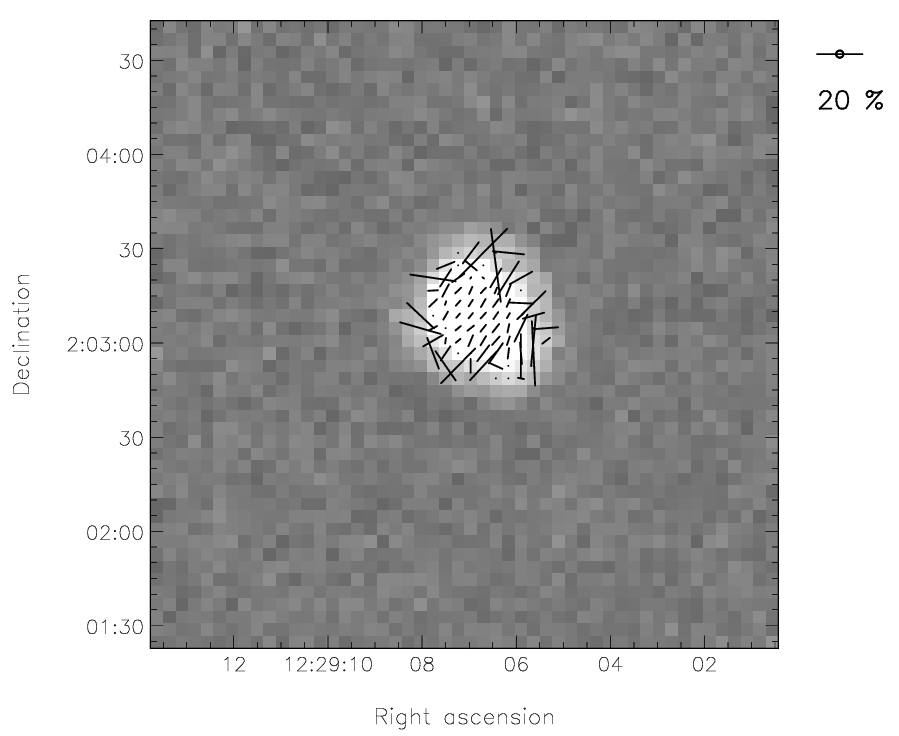
\includegraphics[width=0.75\linewidth]{sc22-kappa-plots-plot3.png}
\caption [Vector map with negative image in polplot]{Result from
  Example 1: Producing a vector map over a negative image.\label{fig:kappa-plot3}}
\end{center}
\end{figure}


\section{TOPCAT}

Catalogues produced by \poltwomap\ can be explored using the popular
\topcat\ catalogue browser (see \url{http://www.starlink.ac.uk/topcat/}). For
instance:

\begin{terminalv}
% topcat -f fits mycat.FIT
\end{terminalv}

Unlike the other tools described above, \textsc{Topcat} cannot visualise the
catalogue as a set of vectors. However, it goes well beyond the
facilities of the other tools in allowing you to explore correlations
between different quantities in the catalogue via 2- and 3-dimensional
scatter plots - see Figure~ \ref{fig:topcat}. It can also be used to
cross-correlate two different
catalogues, create subsets of the catalogue, create new columns
containing related quantities, \emph{etc}. It also allows the modified
catalogue to be saved to a new catalogue file on disk. However, beware
that any new catalogue will not contain the WCS information required
by other Starlink applications to perform WCS-related operations such as
displaying annotated axes and aligning data-sets. However, this WCS
information can be copied back into the new catalogue using the
``\xref{polwcscopy}{sun223}{POLWCSCOPY}'' command. See Section~\ref{sec:wcscopy}.

\begin{figure}[t!]
\begin{center}
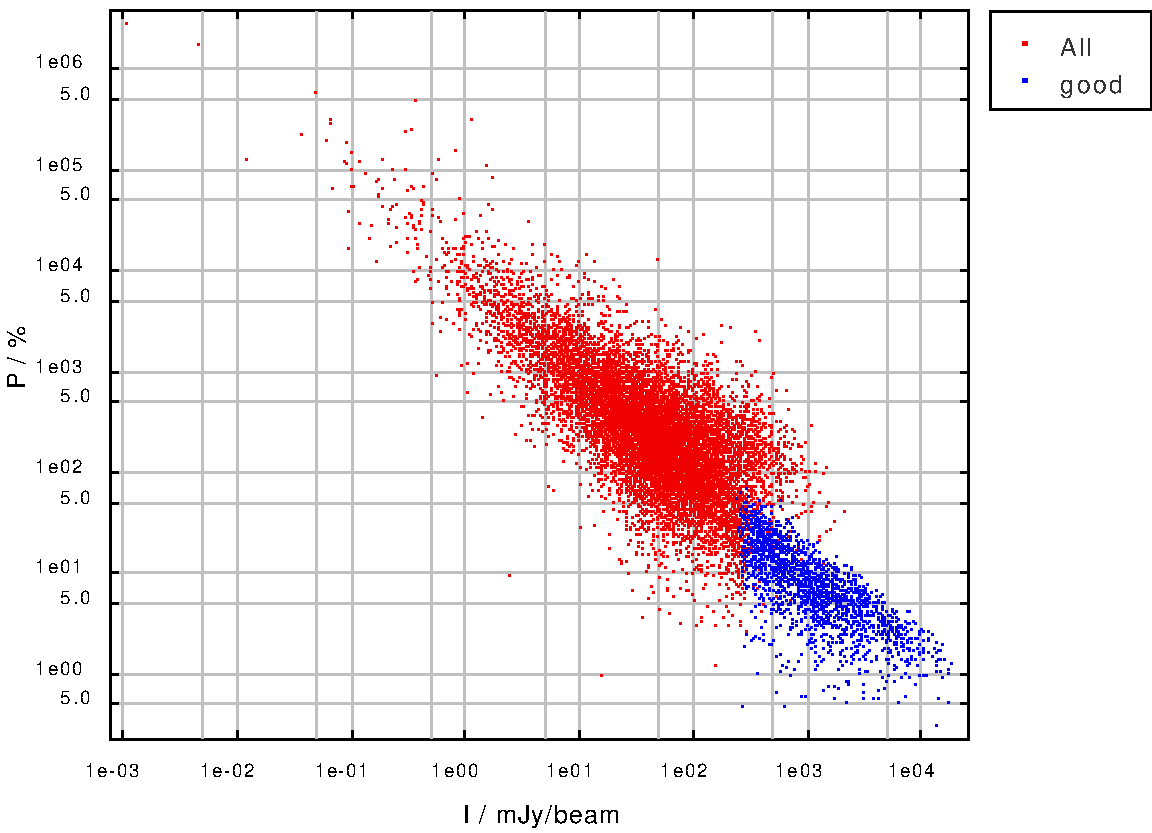
\includegraphics[width=0.75\linewidth]{sc22-topcat}
\caption [A TOPCAT scatter plot]{A scatter plot of fractional polarisation (P)
against total intensity (I) produced by \textsc{Topcat}. High signal-to-noise points
(I>10.DI) are shown in blue.\label{fig:topcat}}
\end{center}
\end{figure}

